\documentclass[a4paper,10pt]{article}
\usepackage[margin=12mm,top=15mm,bottom=15mm]{geometry}
\usepackage{newtxmath}
\usepackage[no-math]{fontspec}
\setmainfont{TeX Gyre Termes}
\usepackage{graphicx,booktabs,tabularx,array,makecell,caption}
\captionsetup{font=small,labelfont=bf,labelsep=period}
\usepackage[backend=biber,style=numeric-comp,sorting=none,giveninits=true,maxbibnames=5,doi=false,url=false,isbn=false,
  date=year]{biblatex}
\addbibresource{../tailieu.bib}
\DeclareSourcemap{\maps[datatype=bibtex]{\map{\step[fieldset=addendum,null]}}}
\renewcommand{\thefigure}{F\arabic{figure}}
\renewcommand{\thetable}{T\arabic{table}}
% labels of the manuscript that the captions cite
\makeatletter
\newcommand{\fakelabel}[2]{\expandafter\gdef\csname r@#1\endcsname{{#2}{}{}{}{}}}
\makeatother
\fakelabel{thm:p3-pair}{1}
\fakelabel{prop:p3-info}{9}
\fakelabel{sec:infoloop}{6.8}
\fakelabel{sec:sens}{6.9}
\fakelabel{sec:bench}{6.1}
\fakelabel{sec:certs}{2.4}
\title{Conformal mission reserve certificates: figures and tables}
\author{Overview of the figures and tables of the manuscript, with their captions}
\date{\today}
\begin{document}
\maketitle
\noindent Sources of the final figures and tables, all in \texttt{P3\_hinh\_bang/}:
\begin{itemize}\setlength{\itemsep}{0pt}
\item F1: \texttt{F1\_cau\_truc.tex} (TikZ, compiled with xelatex);
\item F2 and F4--F9: \texttt{P3\_mophong/hinh\_cuoi.py}; F3: \texttt{P3\_kiemtoan/hinh\_cuoi\_f3.py};
\item T1, T3 and T5: \texttt{P3\_mophong/bang\_cuoi.py}, one table environment per file, for \verb|\input| in the
manuscript; Tables S2--S10 of the Supplementary Material come from the same script.
\end{itemize}
Figures are vector PDF at print size (90, 140 or 190~mm wide, text 7--8~pt), with 300~dpi PNG previews. Every number
is read from the saved results; nothing is re-simulated. In the manuscript, F1--F9 are Figures 1, 3, 2, 4, 5, 7, 8, 9 and 6,
and T1, T5 and T3 are Tables 2--4. Since 18/10/2026 the case study uses the 3.3~kV converter and certificates per module.
\clearpage
\begin{figure}[p]
\centering
\makebox[\textwidth][c]{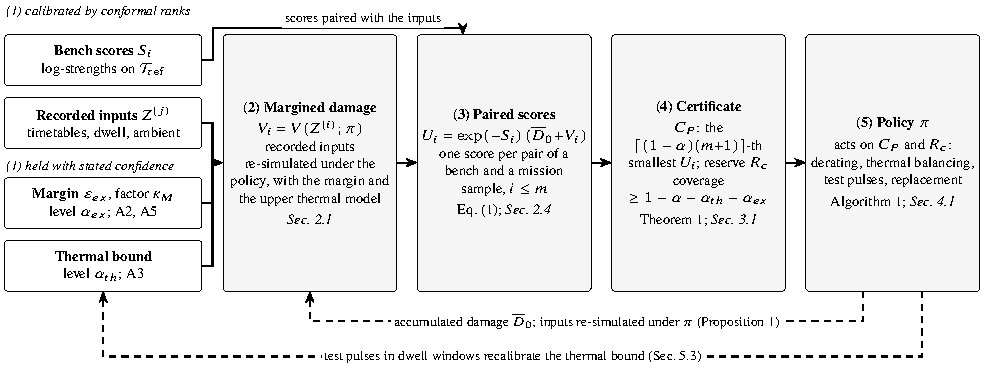
\includegraphics{F1.pdf}}
\caption{Structure of the paired certificate. White boxes: inputs; shaded boxes: computed quantities, each with a
one-line statement and the equation, result and section that give it. Solid arrows: computation; dashed arrows: policy
feedback.}
\label{fig:p3-F1}
\end{figure}

\begin{figure}[p]
\centering
\makebox[\textwidth][c]{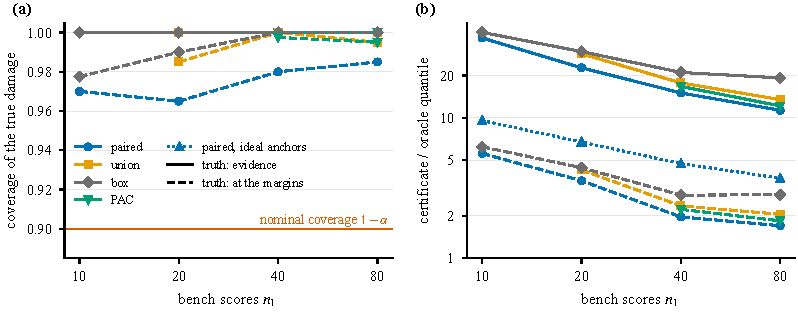
\includegraphics{F2.pdf}}
\caption{Paired, union, box and PAC (training-conditional) certificates for a new leg (both modules) against the
number of bench scores $n_1$ ($n_2=100$, $\alpha=0.10$). (a) Coverage of the true damage; red line: $1-\alpha$. (b)
Median certificate relative to the oracle quantile. Solid: evidence truth; dashed: truth at the margins; dotted:
paired certificate with ideal anchor tests.}
\label{fig:p3-F2}
\end{figure}

\begin{figure}[p]
\centering
\makebox[\textwidth][c]{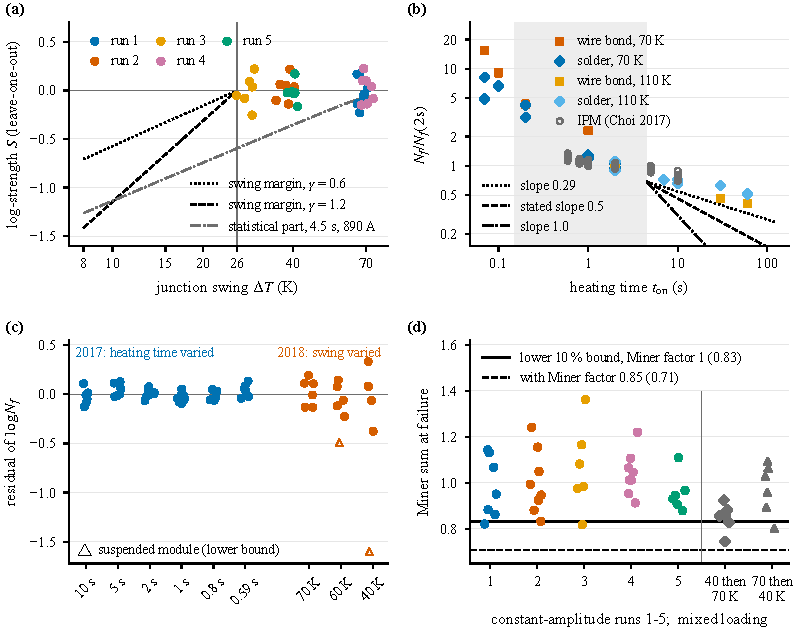
\includegraphics{F3.pdf}}
\caption{Empirical tests of the assumptions on digitized power-cycling data. (a) Leave-one-out log-strength of the
modules of Hernes et al.~\cite{hernes2021} against the swing, by run, with swing margin below 26~K ($\gamma=0.6$ and stated 1.2)
and statistical part of the model at 4.5~s and 890~A. (b) Life against heating time, or swing duration, in tests that
vary it alone~\cite{junghaenel2017mr,choi2017}, normalized at 2~s, with stated slope $\gamma_t=0.5$ and its
sensitivity range; shading: tested range of the model. (c) Residual log-lives of one intelligent power module (IPM) type in two campaigns
\cite{choi2017,choi2018mr}; triangles: suspended modules. (d) Miner sum at failure of the mixed-loading modules of
Hernes et al.~\cite{hernes2021pcim} against the constant-amplitude runs, with the conformal lower 10\,\% bound for $\kappa_M=1$ and
0.85.}
\label{fig:p3-F3}
\end{figure}

\begin{figure}[p]
\centering
\makebox[\textwidth][c]{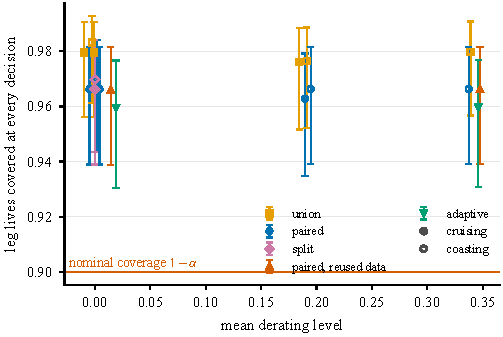
\includegraphics{F4.pdf}}
\caption{Coverage per leg life under feedback: share of the 300 lives per run in which every certificate of both
modules covers the true damage (truth at the margins, $\alpha=0.10$; Wilson 95\,\% intervals), against the mean
derating level under the pass/fail, fixed and reserve rules. Filled:
cruising; open: coasting; red line: $1-\alpha$.}
\label{fig:p3-F4}
\end{figure}

\begin{figure}[p]
\centering
\makebox[\textwidth][c]{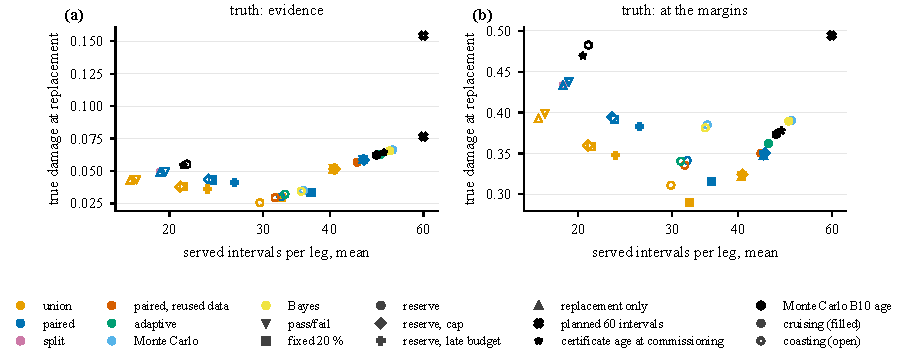
\includegraphics{F5.pdf}}
\caption{True damage at replacement against served intervals per leg (mean over lives without failure; 300
common lives per truth and driving strategy). (a) Evidence truth; (b) truth at the margins. Color: certificate (black:
baseline); marker: policy or baseline; filled: cruising, open: coasting.}
\label{fig:p3-F5}
\end{figure}

\begin{figure}[p]
\centering
\makebox[\textwidth][c]{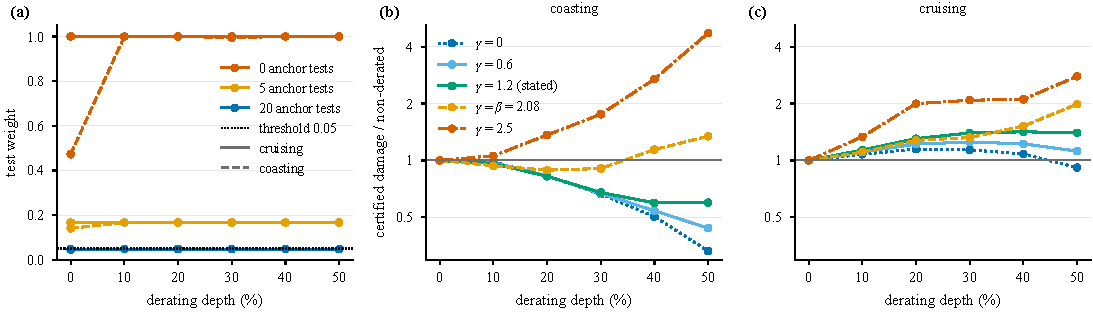
\includegraphics{F6.pdf}}
\caption{Collapse by caution on the missions: derating makes the weighted certificate infinite unless anchor tests
cover every derating level. (a) Weight $p_{n_1+1}$ of the test point in weighted calibration
against derating depth, without and with anchor tests at the loading of each derating level (anchors fixed at full
load: Table~S27), cruising (solid) and coasting (dashed);
the weighted strength quantile is infinite while the weight exceeds $\alpha_S=0.05$. (b, c) Certified damage of the
leg in the coming interval relative to the non-derated value, coasting and cruising, for swing-margin slopes
$\gamma$ below, at and above $\beta=2.08$.}
\label{fig:p3-F6}
\end{figure}

\begin{figure}[p]
\centering
\makebox[\textwidth][c]{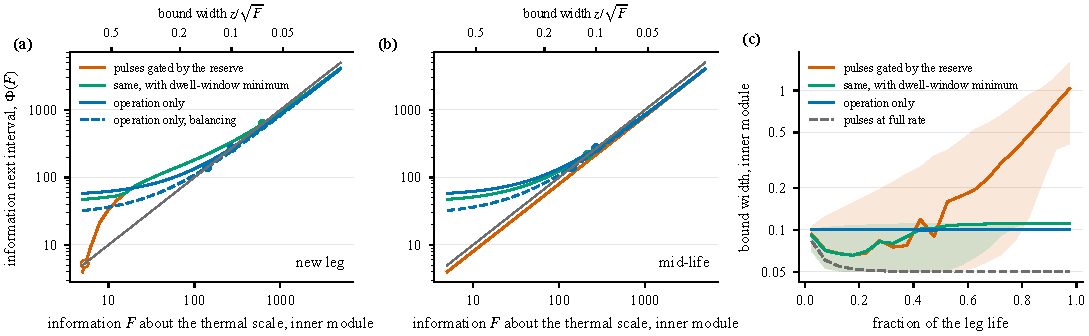
\includegraphics{F7.pdf}}
\caption{Information loop of the thermal bound of the inner module (evidence truth, median over 100 worlds): pulses
withheld at low reserve can starve the bound of information, and 60 counted dwell-window pulses per interval prevent
this. (a, b)
Next-interval information $\Phi(F)$ against present information $F$, for a new module and at mid-life, for pulses
withheld at low reserve, with at least 60 dwell-window pulses per interval, and from operation only (with and without
balancing). Dots: fixed points (open: unstable); gray: $\Phi(F)=F$. (c) Bound width over module life: median and
10--90\,\% band; gray dashed: 300 pulses per interval.}
\label{fig:p3-F7}
\end{figure}

\begin{figure}[p]
\centering
\makebox[\textwidth][c]{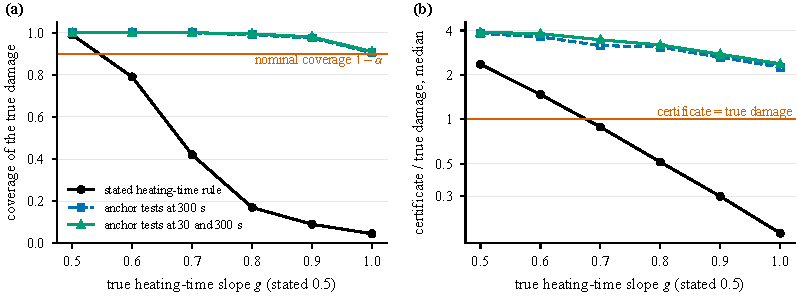
\includegraphics{F8.pdf}}
\caption{Exceedance of the stated heating-time margin: both true heating-time slopes, below and above 60~s, are raised
to $g$, from the stated 0.5 to 1.0, the truth being at the other margins ($n_1=40$, $\alpha=0.10$). (a) Coverage of
the true damage; red line: $1-\alpha$. (b) Median certificate relative to the true damage. Circles: stated rule;
squares and triangles: five anchor tests per anchor time.}
\label{fig:p3-F8}
\end{figure}

\begin{figure}[p]
\centering
\makebox[\textwidth][c]{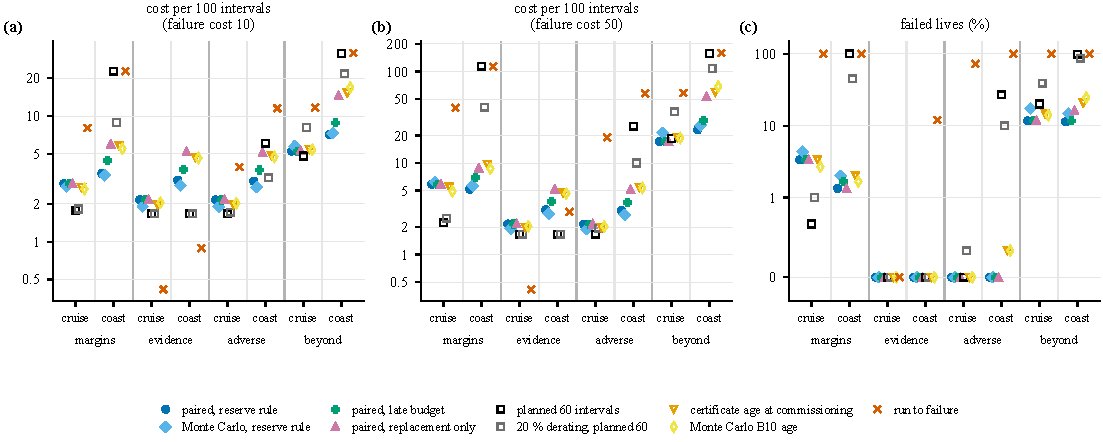
\includegraphics{F9.pdf}}
\caption{(caption in the manuscript)}
\label{fig:p3-F9}
\end{figure}

\clearpage
\begin{table}[tbp]
\centering
\caption{Sources of uncertainty in the end-of-interval damage, the data that inform them, and how each enters the
certificate. Labels are observable when the quantity itself can be measured on the population or the mission before the
decision.}
\label{tab:p3-T1}
\footnotesize
\begin{tabularx}{\textwidth}{@{}>{\raggedright\arraybackslash}p{2.3cm}>{\raggedright\arraybackslash}X
>{\raggedright\arraybackslash}p{3.3cm}>{\raggedright\arraybackslash}X>{\raggedright\arraybackslash}p{3.4cm}@{}}
\toprule
Source & Enters through & Labels observable & Data in the case study & Treatment \\
\midrule
Strength scatter of the device population & log-strength $S$ of a device on the reference conditions
$\mathcal T_{\mathrm{ref}}$ & yes: cycles to failure of bench devices at tested conditions & 34 modules in five runs
\cite{hernes2021} & calibrated: ranks of the scores, level $\alpha$ (paired)
or $\alpha_S$ (union) \\
\addlinespace
Mission variability & inputs $Z$ of a maintenance interval: timetable, dwell times, ambient & yes: recorded intervals,
re-simulated under the deployed policy & 112 days of a high-speed corridor \cite{zhang2022hsr} & calibrated: paired with the scores (level $\alpha$) or own quantile (level $\alpha_V$) \\
\addlinespace
Lifetime extrapolation and damage accumulation & margin $\varepsilon_{ex}(x)$ on cycle lives off
$\mathcal T_{\mathrm{ref}}$ (swing, heating time, current, minimum temperature, statistical part) and Miner factor
$\kappa_M$ & no: no life is observed at field conditions (low swing, long heating time) before the decisions & published
single-factor and mixed-loading tests \cite{junghaenel2017mr,choi2017,choi2018mr,hernes2021pcim,choi2017apec}; solder
fatigue under long dwell \cite{engelmaier1983} & stated with confidence $1-\alpha_{ex}$ (Table~\ref{tab:p3-T5});
anchor tests at field heating times replace the largest component \\
\addlinespace
Thermal response & upper thermal model used in the margined damage $V$ & partly: junction rise measured with test
pulses in dwell windows and in operation & dwell windows of the timetable; thermal path degraded by 20--40\,\% at end
of life (assumed) & stated with confidence $1-\alpha_{th}$; recalibrated each interval (Section~\ref{sec:infoloop}) \\
\bottomrule
\end{tabularx}
\end{table}

\begin{table}[tbp]
\centering
\caption{Coverage and tightness of a single certificate for a new leg ($n_2=100$ recorded intervals, 200
repetitions per cell, each with the outer and the inner module): coverage of the true end-of-interval damage and median
ratio of the certificate to the oracle quantile of the true damage, over both modules.}
\label{tab:p3-T3}
\footnotesize
\setlength{\tabcolsep}{3.2pt}
\begin{tabular*}{\textwidth}{@{\extracolsep{\fill}}lcccccccccc@{}}
\toprule
& \multicolumn{8}{c}{Truth at the margins} & \multicolumn{2}{c}{\makecell{Evidence truth,\\ratio, $\alpha=0.10$}} \\
\cmidrule(lr){2-9}\cmidrule(l){10-11}
& \multicolumn{2}{c}{$\alpha=0.10$, $n_1=20$} & \multicolumn{2}{c}{$\alpha=0.10$, $n_1=40$}
& \multicolumn{2}{c}{$\alpha=0.05$, $n_1=40$} & \multicolumn{2}{c}{$\alpha=0.01$, $n_1=40$} & $n_1=20$ & $n_1=40$ \\
\cmidrule(lr){2-3}\cmidrule(lr){4-5}\cmidrule(lr){6-7}\cmidrule(lr){8-9}
Certificate & cov. & ratio & cov. & ratio & cov. & ratio & cov. & ratio & & \\
\midrule
box & 0.990 & 4.41 & 1.000 & 2.81 & 1.000 & 2.58 & 1.000 & 2.07 & 29.60 & 21.03 \\
Monte Carlo & 0.965 & 3.33 & 0.983 & 1.91 & 0.993 & 1.88 & 1.000 & 1.76 & 21.37 & 14.70 \\
Bayes & 0.970 & 3.38 & 0.983 & 1.93 & 0.995 & 1.91 & 1.000 & 1.80 & 21.84 & 14.85 \\
union & 0.985 & 4.25 & 1.000 & 2.36 & 1.000 & 2.57 & 1.000 & $\infty$ & 28.53 & 17.72 \\
paired & 0.965 & 3.56 & 0.980 & 1.97 & 0.998 & 2.04 & 1.000 & $\infty$ & 22.69 & 15.02 \\
PAC & 1.000 & $\infty$ & 0.998 & 2.23 & 1.000 & $\infty$ & 1.000 & $\infty$ & $\infty$ & 16.72 \\
paired, ideal anchor tests$^{\dagger}$ & -- & -- & -- & -- & -- & -- & -- & -- & 6.72 & 4.72 \\
oracle$^{\dagger}$ & 0.900 & 1.00 & 0.900 & 1.00 & 0.950 & 1.00 & 0.985 & 1.00 & 1.00 & 1.00 \\
\bottomrule
\end{tabular*}

\smallskip
\begin{minipage}{\textwidth}\scriptsize
$\infty$: infinite in every repetition (coverage then trivial). Under the evidence truth every certificate except
the oracle covers 1.000 (ideal anchor tests: 1.000). Calibrated part of the paired certificate at the margins: 0.917 and 0.922 at $\alpha=0.10$, 0.955 at $\alpha=0.05$. Monte Carlo standard error of the paired
coverage at the margins ($n_1=40$, $\alpha=0.10$; both modules of a repetition share a bench): 0.008.
$^{\dagger}$Uses the truth; for analysis only.
\end{minipage}
\end{table}

\begin{table}[tbp]
\centering
\caption{Stated extrapolation margin of the case study. (a) Components, values, evidence and sensitivity ranges; the
thermal bound, held at its own level $\alpha_{th}$, is listed for completeness. (b) Margin budget in log units (log of
the factor on damage) for two traction cycles and for the damage-weighted journey, with the calibrated part for
comparison.}
\label{tab:p3-T5}
\footnotesize
\textit{(a) Components}\\[2pt]
\begin{tabularx}{\textwidth}{@{}>{\raggedright\arraybackslash}p{2.6cm}>{\raggedright\arraybackslash}p{3.5cm}
>{\raggedright\arraybackslash}p{2.0cm}>{\raggedright\arraybackslash}X>{\raggedright\arraybackslash}p{2.9cm}@{}}
\toprule
Component & Rule & Stated value & Evidence & Sensitivity (Section~\ref{sec:sens}) \\
\midrule
Statistical error of $N^{\mathrm{mod}}$ off the tested conditions & one-sided bound on $\log V$ of the interval along
its gradient, relative to the tested conditions & Student $t_{0.95}$; $\alpha_{stat}=0.05$ within $\alpha_{ex}$, approximate &
fit covariance; simulated coverage 0.910--0.975 & Scheff\'e ellipsoid; none \\
\addlinespace
Swing below $\Delta T_{\mathcal T}=26$~K & $\gamma\log(\Delta T_{\mathcal T}/\Delta T)$ & $\gamma=1.2$ & swing exponent
changing from 4.42 to 3.21 at a mechanism switch \cite{scheuermann2018} & $\gamma\in\{0,0.6,2.08\}$;
$\Delta T_{\mathcal T}=68$~K \\
\addlinespace
Heating time 4.5--60~s & $N^{\mathrm{mod}}$ at 4.5~s plus $\gamma_t\log(t_{\mathrm{on}}/4.5\,\mathrm{s})$ &
$\gamma_t=0.5$ & slopes $-0.19$ (solder) and $-0.27$ (wire bond) at 2--60~s \cite{junghaenel2017mr}; $-0.14$
\cite{choi2017}; $-0.463$ (CIPS08 \cite{bayerer2008}); the long-heating-time tests lack a baseplate &
$\gamma_t\in\{0.29,1.0\}$ \\
\addlinespace
Heating time above 60~s & same slope, not capped & $\gamma_t=0.5$ & solder fatigue grows with the dwell up to hours,
12--20 times from 1~min to 10~h \cite{engelmaier1983}, against 24.5 for $\gamma_t=0.5$; no single-factor test above
60~s & cap at 60~s; slope 0.27 above 60~s \\
\addlinespace
Current & clipped to 890--1250~A; no credit below 890~A & -- & current exponent not identified apart from the
heating-time exponent (correlation 0.99); field current at most 554~A & -- \\
\addlinespace
Minimum temperature above 60~$^\circ$C & Arrhenius term, activation energy $E_a$; no credit below 60~$^\circ$C & $E_a=0.159$~eV & 0.069--0.159~eV
for wire bond and solder \cite{scheuermann2018}; 0.111~eV (CIPS08); 0.132~eV for silicon carbide \cite{hoffmann2023} &
$E_a=0.111$~eV \\
\addlinespace
Miner's rule & $-\log\kappa_M$ & $\kappa_M=0.85$ & 0.85 and 0.97 for the two load orders \cite{hernes2021pcim};
0.84 and 0.93 under mixed swing durations \cite{choi2017apec}; 1.08 and 1.01 for block and alternating sequences
\cite{zeng2019} & $\kappa_M=1$ \\
\midrule
Thermal bound (level $\alpha_{th}$) & upper scale of the modeled junction rise, stated or recalibrated each interval
(Section~\ref{sec:infoloop}) & stated 1.10 & field degradation of the thermal path, 20--40\,\% at end of life &
confidence, forgetting, pulses and drift (Table~S9) \\
\bottomrule
\end{tabularx}

\medskip
\textit{(b) Margin budget (log units)}\\[2pt]
\begin{tabular*}{\textwidth}{@{\extracolsep{\fill}}lcccccccc@{}}
\toprule
& Calibrated & \multicolumn{5}{c}{Stated} & & \\
\cmidrule(lr){2-2}\cmidrule(lr){3-7}
Cycle or mission & $-q_S$ & statistical & swing & heating time & $T_{\min}$ & Miner & stated total & factor \\
\midrule
40~K, 90~s, $T_{\min}$ 60~$^\circ$C & 0.17 & 0.53 & 0.00 & 1.50 & 0.00 & 0.16 & 2.19 & 9 \\
10~K, 90~s, $T_{\min}$ 70~$^\circ$C & 0.17 & 1.67 & 1.15 & 1.50 & 0.16 & 0.16 & 4.64 & 104 \\
journey, cruising, chip D1$^{*}$ & 0.17 & 1.10 & 0.33 & 2.49 & 0.00 & 0.16 & 4.08 & 59 \\
\bottomrule
\end{tabular*}

\smallskip
\begin{minipage}{\textwidth}\scriptsize
(b) Calibrated part: lower 10\,\% quantile of the 34 leave-one-out log-strengths; statistical part with the half
split of the bench data, for the cycles with the normal quantile 1.645 in place of $t_{0.95}$. $^{*}$Damage-weighted over
the cruising journey without derating, the critical chip of the leg; heating time 1.28 for 4.5--60~s and 1.21 above
60~s; the statistical part is the median ratio of the interval damage with and without it over 40 half splits.
\end{minipage}
\end{table}

\clearpage
\printbibliography
\end{document}
